%\motto{Use the template \emph{chapter.tex} to style the various elements of your chapter content.}
\chapter{Quantensoftware und Programmierung}
\label{programming} % Always give a unique label
% use \chaptermark{}
% to alter or adjust the chapter heading in the running head

\chapterauthor{Konrad Maywald, Daniel Purtov, Dennis Schweigert, Tom Williard}

\abstract{some abstract}

\section{Programmiermodelle in der Quanteninformatik}

\subsection{Gate-basiertes Paradigma (Quantum Circuit Model)}
Das Gate basierte Paradigma oder auch Quantenschaltkreis Modell (engl. Quantum Circuit Model) genannt, ist das Standardmodell für die Programmierung von Quantenprogrammen. Daher wird es auch häufig als das am weitesten verbreitete Paradigma in der Quanteninformatik zur Beschreibung und Realisierung von Quantenalgorithmen bezeichnet. In diesem Modell werden die Quantenprogramme als Schaltkreise (engl. Quantum circuits) dargestellt. Diese bestehen aus einer Sequenz von unitären Quanten Gattern, welche auf Qubits angewendet werden. 

Strukturell orientiert sich das Quantenschaltkreismodell an klassischen digitalen Schaltungen. Klassische Schaltkreise bestehen aus Leitungen, Gattern und klassischen Bits mit den Zuständen 0 und 1. Ganz analog dazu bestehen Quantenschaltkreise aus Qubit-Leitungen und Gattern und Quantenbits (Qubits). Jede Leitung repräsentiert dabei ein Qubit und jedes Gatter eine unitäre Transformation auf eines oder mehrere Qubits. Die Struktur des Quantenschaltkreis wird genauso wie bei digitalen Schaltungen meist visuell dargestellt, um die Reihenfolge der angewendeten Operationen und die daran beteiligten Qubits zu verdeutlichen. 

Folgende Abbildung zeigt typische elementare Gates, welche für die Konstruktion von Quantenschaltkreisen verwendet, werden: 
\begin{figure}
    \centering
    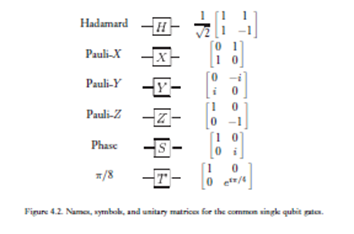
\includegraphics[width=0.5\linewidth]{Qubit Gates.png}
    \caption{Qubit Gates}
    \label{fig:enter-label}
\end{figure}

\begin{itemize}
    \item Das Hadamard-Gate (H) bringt Qubits aus Ihren Basiszuständen in eine Superposition 
    \item Das CNOT-Gate (Controlled-Not), ist ein zwei Qubit Gate, welches als zentraler Bestandteil der Quantenverschränkung funktiert, es verschränkt sozusagen zwei Qubits miteinander 
    \item Neben diesen beiden sehr wichtigen Gates gibt es auch noch die Pauli-X, -Y. und -Z Gates, sowie Phasengatter, T-Gate  und weitere 
\end{itemize}
Werden mehrerer dieser Gatter nacheinander auf ein Qubit Register angewendet, bildet sich daraus ein Quanten-Schaltkries, welcher als gesamter Algorithmus verstanden werden kann.
\subsection*{Bekannte Quantenalgorithmen basierend auf dem Quantenschaltkreismodell}
Das Quantenschaltkreismodell dient als Grundlage für mehrere bekannte Quantenalgorithmen dazu zählen folgende: (siehe auch (\autoref{basic_algorithms}))
\subsubsection*{1) Shor's Algorithmus}
Der Shor Algorithmus führt eine effiziente Primfaktorzerlegung großer Zahlen durch, was klassische Verschlüsselungsverfahren wie RSA bedroht. Der Algorithmus verwendet die Quantum Fourier Transformation (QFT) und periodenfindende Subroutinen innerhalb des Circuit-Models. (siehe auch (\autoref{first:shor-algorithm})
\subsubsection*{2) Grover´s Algorithmus}
Der Grover Algorithmus dient zur Suche eines Eintrags in einer unstrukturierten Datenbank mit einer quadratischen Beschleunigung gegenüber klassischen Verfahren.
Der Algorithmus basiert auf Rotation in einem zweidimensionalen Unterraum, dargestellt als wiederholte Anwendung von sogenannten Grover-Iterationen, realisiert durch Gates im Circuit-Modell. (ausführliche Erklärung: (\autoref{sec:grover-algorithm})) 

\subsubsection*{3) Regev}
Regevs Arbeiten zum LWE-Problem beinhalten eine theoretische Quantenreduktion, die sich vollständig im gate-basierten Modell realisieren lässt. Die dafür erforderlichen Operationen – wie das Erzeugen von Superpositionen, die Anwendung der Quanten-Fouriertransformation sowie die Verarbeitung von Messresultaten – sind mit klassischen Quanten-Gattern (z.B. Hadamard-, CNOT- und Phasengattern) darstellbar. Auch wenn Regevs Reduktion primär theoretischer Natur ist und keine praktischen Implementierungen wie Shor oder Grover hat, zeigen die verwendeten Techniken eine klare Kompatibilität mit dem Quantum Circuit Model.
\textbf{Hier muss ne Leerzeile rein geht aber nicht}
Das gate-basierte Paradigma ist nicht nur ein theoretisches Modell, das man in der Quanteninformatik zur Beschreibung von Algorithmen verwendet – es spielt auch in der Praxis eine zentrale Rolle. So setzt zum Beispiel das Open-Source-Framework Qiskit von IBM genau auf dieses Modell: Quantenprogramme werden dort direkt als sogenannte „Quantum Circuits“ aufgebaut. Diese bestehen aus einer festen Anzahl von Qubits und einer Folge von Operationen, also Gattern, Messungen und Resets – genau wie es im Schaltkreis-Modell vorgesehen ist.
Dass Theorie und Praxis hier so eng zusammenhängen, zeigt, wie wichtig das gate-basierte Modell nicht nur für die Entwicklung von Algorithmen ist, sondern auch für den praktischen Einsatz auf echten Quantencomputern, wie denen von IBM oder Google.

\subsection{Messungsbasiertes Paradigma}
Das messungsbasierte Paradigma, auch bekannt als Measurement-Based Quantum Computing (MBQC) oder one-way quantum computation, stellt eine alternative Architektur zur Implementierung von Quantenalgorithmen dar. Im Gegensatz zum weit verbreiteten Schaltkreis-Modell, bei dem Quanteninformationen durch sequenzielle Anwendung unitärer Gatter verarbeitet werden, basiert MBQC auf einer anderen Grundidee: Der eigentliche Rechenprozess erfolgt nicht durch Gatter, sondern ausschließlich durch gezielte Einzelqubit-Messungen an einem vorbereiteten, verschränkten Vielteilchenzustand – dem sogenannten Cluster-State.
Diese Struktur eröffnet neue Perspektiven auf die Organisation und Steuerung von Quanteninformation. Die gesamte logische Verarbeitung geschieht dabei einseitig – also „one-way“ – da jede Messung irreversibel ist und den gemessenen Qubit-Zustand zerstört. Die Fähigkeit zur universellen Quantenberechnung wird dabei vollständig durch die Verschränkungseigenschaften des vorbereiteten Zustands sowie die geschickte Wahl und Abfolge der Messungen realisiert.
\subsection*{Struktur und Erzeugung von Cluster-States}
Zentrale Ressource des MBQC ist der Cluster-State, ein hochgradig verschränkter Quantenzustand mehrerer Qubits. Formal gehört der Cluster-State zur Klasse der Graphenzustände. Diese Zustände lassen sich durch mathematische Graphen beschreiben, in denen Knoten einzelnen Qubits entsprechen und Kanten die Verschränkungen zwischen ihnen darstellen.

Die Erzeugung eines solchen Zustands erfolgt in zwei Schritten:
\begin{enumerate}
    \item 	Zunächst werden alle Qubits in den Zustand $|+\rangle = \frac{1}{\sqrt{2}}(|0\rangle + |1\rangle)$ gebracht.
    \item 2.	Anschließend wird auf jedes benachbarte Qubitpaar (gemäß der Graphstruktur) ein kontrolliertes Phasengatter $U_{PG}=diag(1,1,1,-1)$ angewendet.
\end{enumerate}
Der so erzeugte Zustand $|G\rangle$, wobei G der zugrundeliegende Graph ist, besitzt die gewünschten Verschränkungseigenschaften, um ihn als Rechenressource im MBQC zu verwenden. Besonders der zweidimensionale (2D) Cluster-State hat sich hierbei als universell erwiesen, d.h. als hinreichend mächtig für die Implementierung beliebiger Quantenalgorithmen.
\subsection*{Rechenmodell und Algorithmus Implementierung}
Eine MBQC-Berechnung lässt sich in einem schematischen Ablauf darstellen, der vier grundlegende Schritte umfasst:
\begin{enumerate}
    \item \textbf{Initialisierung:} Vorbereitung eines ausreichend großen 2D-Cluster-States, der unabhängig vom konkreten Algorithmus erzeugt wird.
    \item \textbf{Kodierung des Algorithmus durch Messmuster:} Die Berechnung wird durch eine Sequenz von Einzelqubit-Messungen in ausgewählten Basen realisiert. Dabei bestimmt das Muster der Messungen (also deren Reihenfolge und jeweilige Basis) die Art der durchgeführten logischen Operationen.
    \item \textbf{Adaptive Steuerung:} Die Wahl der Messbasis für spätere Schritte kann von den Ergebnissen vorheriger Messungen abhängen. Diese Feedforward-Kontrolle wird durch eine klassische Recheneinheit übernommen.
    \item \textbf{Ausgabezustand:} Das Endresultat der Quantenberechnung ist entweder in den verbleibenden nicht gemessenen Qubits codiert oder ergibt sich aus den Messergebnissen selbst. Die resultierenden Zustände unterscheiden sich höchstens durch lokale Pauli-Operationen.
\end{enumerate}
Ein bemerkenswertes Merkmal dieses Modells ist, dass trotz der inhärenten Zufälligkeit der einzelnen Messergebnisse (aufgrund des quantenmechanischen Messprozesses) der gesamte Rechenvorgang deterministisch kontrolliert und wiederholbar bleibt – vorausgesetzt, das Feedforward wird korrekt berücksichtigt 
\subsection*{Exemplarische Anwendungen}
Das Potential des MBQC lässt sich gut an ausgewählten Beispielen verdeutlichen. Eines der grundlegendsten Konzepte ist das Teleportationsprotokoll, das im Kontext des MBQC zeigt, wie Quanteninformation durch Messungen effektiv von einem Teil des Clusters zum anderen übertragen werden kann. Dieses Prinzip bildet die Basis für viele weiterführende Techniken, darunter auch die Realisierung effektiver logischer Gatter allein durch Messungen.
Darüber hinaus lassen sich bekannte Algorithmen wie der Shor-Algorithmus zur Faktorisierung großer Zahlen oder der Grover-Algorithmus zur Datenbanksuche in messungsbasierten Varianten formulieren. Diese benötigen lediglich eine geeignete Struktur des zugrunde liegenden Cluster-States sowie eine korrekt gewählte Messstrategie, um dieselbe Funktionalität wie im Schaltkreis-Modell zu erreichen. Damit zeigt sich die formale Äquivalenz der beiden Paradigmen – bei grundlegend unterschiedlicher Umsetzung.

\subsection{Adiabatisches Paradigma (Quantum Annealing)}
Ein weiteres Modell zur Realisierung von Quantenalgorithmen ist das adiabatische Paradigma, welches auch als Quantum Annealing bezeichnet wird. Das Adiabatischen Modell basiert auf der Idee, ein Quantensystem durch eine langsame, kontinuierliche Änderung eines Hamiltonians gezielt in seinen Grundzustand zu führen. Die gesuchte Lösung des Modells ist in diesem Grundzustand markiert. Genau in dieser Art unterscheidet sich das Quantum Annealing auch vom Gate oder messungsbasierten Modell. 
Das Grundprinzip des Modells besteht darin, dass man das Quantensystem zunächst in einem leicht vorbereiteten Anfangszustand hält. Dieser entspricht dem Grundzustand eines sogenannten Treibenden Hamiltonians $H_D$. Dieser Hamiltonian kann z.B. ein transversales Feld enthalten, das alle Qubits gleichmäßig beeinflusst. Im Laufe des Algorithmus wird dann schrittweise der Problem-Hamiltonian $H_P$ zugeschaltet, dieser enthält die Struktur des zu lösenden Problems. Die Gesamtentwicklung erfolgt über einen zeitabgängigen Hamiltonian, der folgenden Form:
$$
H(t) = A(t) \cdot H_D + B(t) \cdot H_P
$$
Die beiden Funktionen A(t) und B(t) steuern, wie stark der jeweilige Hamiltonian zu einem bestimmten Zeitpunkt t wirkt. Am Anfang dominiert hierbei HD und am Ende HP. Das System bleibt nach dem adiabatischen Theorem während des gesamten Prozesses im jeweiligen Grundzustand, wenn die Änderungen langsam genug erfolgen. Am Ende wird die gesuchte Lösung, also der Grundzustand von $H_P$ erreicht.
Die Hamiltonian dürfen mit einer Geschwindigkeit geändert werden, die stark vom sogenannten Energieabstand (Gap) zwischen dem Grundzustand und dem ersten angeregten Zustand abhängt. Je kleiner dieser Abstand ist, desto langsamer muss die Änderung erfolgen, um unerwünschte Übergänge in angeregte Zustände zu vermeiden. 
Das Quantum Annealing eignet sich besonders gut für kombinatorische Optimierungsprobleme, da viele davon auf sogenannte Ising-Modelle abgebildet werden können. Ein Beispiel für ein Problem-Hamiltonian ist folgendes:
$$
H_P = \sum_{i,j} J_{ij}\sigma_i^z\sigma_j^z + \sum_i h_i\sigma_i^z
$$
Die Kopplungsterme $J_{ij}$ und die lokalen Felder $h_i$ kodieren hierbei die jeweilige Problemstruktur.
Es gibt verschiedene Problemklassen, welche durch Quantum Annealing gelöst werden können, zu den typischen gehören unter anderem Folgende Beispiele: 
\begin{itemize}
    \item \textbf{Max-Cut: }Bei Max-Cut wird ein Graph aufgeteilt in zwei Teilmengen, sodass die Kantensumme zwischen den beiden Mengen maximal wird 
    \item 	\textbf{k-Clique:} Bei der k-Clique-Suche geht es darum, vollständige Teilgraphen mit genau k Knoten zu finden, also Untergruppen, in denen jeder Knoten mit jedem anderen verbunden ist 
    \item \textbf{Graph Coloring: }Beim Graph Coloring sollen Knoten eines Graphen mit möglichst wenigen Farben so eingefärbt werden, dass benachbarte Knoten unterschiedliche Farben erhalten 
    \item \textbf{Ising-Modell-Minimierung:} Hier wird der Ising-Hamiltonian direkt minimiert. Da sich viele kombinatorische Probleme darauf abbilden lassen, bildet diese Minimierung die Grundlage für zahlreiche Optimierungsaufgaben 
\end{itemize}
Quantum Annealing (QA) verwendet im Gegensatz zum klassischen Simulated Annealing (SA), bei der thermische Fluktuationen benutzt werden, Quantenfluktuationen, insbesondere Quanten-Tunnel, um Energiebarrieren zu überwinden. Das ist vor allem dann ein Vorteil, wenn die Energiebarrieren hoch, aber schmal sind. In genau diesen Fällen kann das Quantum Annealing schneller zu einer optimalen Lösung finden als sein klassischen Gegenstück Simulated Annealing. 
Das adiabatische Paradigma wurde in der Praxis unter anderem durch die Firma D-Wave Systems in Hardware umgesetzt. Die Systeme von D-Wave Systems sind darauf spezialisiert Optimierungsprobleme durch Quantum Annealing zu lösen, also das adiabatische Paradigma technisch zu realisieren. 
\subsection{Hybrid-Paradigma}
Das Hybrid-Paradigma stellt neben dem Gate basierten und adiabatischen Modell einen weiteren wichtigen Ansatz zur Realisierung von Quantenalgorithmen dar. Es ist aus dem Grund besonders interessant, da es sowohl klassische als auch quantenmechanische Bestandteile kombiniert. Konkret bedeutet das, dass die aufwendigen und hardwareintensiven Berechnungen, wie etwa die Manipulation und Messung von Quantenzuständen auf dem Quantencomputer laufen, während Aufgaben wie das Anpassen von Parametern oder das Auswerten von Messergebnissen klassisch bearbeitet werden. Aufgrund dieser Aufgabenteilung lassen sich viele Probleme bereits heutzutage auf existierender Hardware lösen. Das liegt vor allem daran, dass das Hybrid-Paradigma mit relativ kurzen Quantenschaltungen auskommt und keine langen kohärenten Entwicklungen benötigt.
Das Grundprinzip im Hybrid-Paradigma ist immer gleich. Man startet zunächst mit einem Anfangszustand, der mithilfe einer parametrierten Quantenschaltung erzeugt wird. Anschließend wird ein Zielwert gemessen, das kann z.B. eine Energie sein und gibt dann diesen Messwert an den klassischen Computer zurück. Auf diesem wird dann ein Optimierungsalgorithmus ausgeführt, der neue Parameter vorschlägt, mit denen die Quantenschaltung beim nächsten Durchlauf verändert wird. Dieser Prozess wird so lange wiederholt, bis ein gewünschtes Ergebnis erreicht ist. Das erklärte Prinzip kommt in mehreren hybriden Algorithmen zum Einsatz. Im Folgenden werden nun drei bekannte hybride Algorithmen genauer vorgestellt. 
\subsubsection*{1) Variationaler Quanten Eigenlöser (VQE)}
Der variationale Quanten Eigenlöser (engl, variational quantum eigensolver), kurz VQE, ist ein hybrider Algorithmus der Berechnung von Eigenwerten, genauer gesagt zur Bestimmung des Grundzustands eines Hamiltonians verwendet wird. In der Quantenchemie ist das extrem wichtig, da sich damit die Energie eines Moleküls berechnen lässt. Die Idee hinter dem VQE-Algorithmus ist es einen Quantenzustand $|\psi(\theta)\rangle$ vorzubereiten, der von bestimmten Parametern $\theta$ abhängt. Für diesen Zustand wird dann der Erwartungswert einer Energie gemessen, was sich mathematisch durch folgende Formel ausdrücken lässt:
$$
\langle\psi(\theta)|H|\psi(\theta)\rangle
$$
Dieser Ausdruck wird als sogenannte Kostenfunktion verwendet. Das Ziel ist es die Parameter θ so zu verändern, dass die gemessene Energie möglichst klein wird und somit dem Grundzustand des Systems entspricht. Dieser Schritt passiert auf einem klassischen Rechner, der z.B. den Nelder-Mead-Algorithmus oder einen anderen Optimierer nutzt, nicht auf dem Quantencomputer selbst. 
Ein großer Vorteil von VQE ist, dass die benötigten Quantenschaltungen relativ flach bleiben, sie kommen mit wenigen Gattern und kurzen Operationen aus. Diese Tatsache ist besonders für NISQ-Hardware praktisch, da bei dieser jede zusätzliche Operation das Risiko für Fehler erhöht. 
2014 wurde der VQU bereits durch Peruzzo et al, erfolgreich auf einem photonischen Quantenprozessor umgesetzt. Dabei wurde die Bildungskurve des Moleküls He–H⁺ berechnet. Die Energie wurde dabei über ein klassisch-quantisches Zusammenspiel optimiert und das Ergebnis lag innerhalb der chemischen Genauigkeit. Das war bereits ein starker Beweis dafür, dass hybride Algorithmen schon vor über 10 Jahren auf damaliger Hardware praktikabel waren. 

\subsubsection*{2) Quantum Approximate Optimization Algorithm (QAOA)}
Der sogenannte Quantum Approximate Optimization Algorithm (QAOA) ist ein weiterer Algorithmus des Hybrid-Paradigmas und wurde dazu entwickelt, um kombinatorische Optimierungsprobleme zu lösen. Typische Beispiele hierfür sind Max-Cut, k-Clique oder andere Graph Probleme (siehe Kapitel…). Auch QAOA besteht aus einem parametrisierten Quantenschaltkreis und einer klassischen Optimierung, funktioniert jedoch deutlich anders als VQE.
Das Verfahren nutzt zwei Hamiltonians. Einmal einen Probleme-Hamiltonian $H_C$, welcher das zu lösende Problem abbildet (z.B. ein Ising-Modell) und einmal einen sogenannten Mixer-Hamiltonian $H_B$, der typischerweise eine Summe von X-Gattern ist. Ausgehend vom Anfangszustand werden nun abwechselt die Hamiltonian $H_C$ und $H_B$ auf das System angewendet. Daraus ergibt sich dann für eine Schaltungstiefe p folgender QAOA-Zustand: 
$$
|\psi_p(\vec{\gamma}, \vec{\beta})\rangle = e^{-i\beta_p H_B}e^{-i\gamma_p H_C} \dots e^{-i\beta_1 H_B}e^{-i\gamma_1 H_C} |+\rangle^{\otimes N}
$$
Die Parameter $\gamma$ und $\beta$ werden dabei von einem klassischen Optimierer so angepasst, dass die gemessene Erwartung des Zieloperators optimiert wird. Das System bleibt hierbei anders als beim adiabatischen Paradigma nicht unbedingt im Grundzustand, sondern nutzt gezielt nicht-adiabatische Übergänge, um effizient zu besseren Lösungen zu kommen. Damit eignet sich der Algorithmus gut für NISQ-Geräte und kann mit relativ flachen Quantenschaltungen implementiert werden. 

\subsubsection*{3) Quantum Machine Learning}
Das letzte der drei genannten typischen Gebiete in dem hybride Quantenalgorithmen eine wichtige Rolle spielen, ist das sogenannte Quantum Machine Learning. Hierbei kommt es wie der Name schon vermuten lässt zur Verbindung von Quantencomputing und maschinellem Lernen. Auch in diesem Gebiet ist das Hybrid-Paradigma der Standard, weil klassische Daten verarbeitet und mit quantenmechanischen Methoden analysiert werden. 
Hierbei läuft das typische Vorgehen wie folgt ab. Zunächst werden die Eingangsdaten, also z.B. Bilder oder numerische Werte, durch sogenannte Feature Maps in einen Quantenzustand umgewandelt. Anschließend wird dieser Zustand durch eine parametrisierte Quantenschaltung geschickt die als Klassifikator dient. Abschließend wird das Ergebnis auf einem klassischen Computer ausgewertet und der Fehler wird klassisch minimiert. 
Ein Beispiel für Quantum Machine Learning ist der Variational Quantum Classifier (VQC), bei dem die Quantenschaltung so trainiert wird, dass sie zum Beispiel zwischen verschiedenen Klassen unterscheiden kann, wie z.B. zwischen verschiedenen Ziffern in einem Bild. Auch hier wird eine Kostenfunktion (z.B. der Klassifikationsfehler) iterativ durch einen klassischen Optimierer minimiert. 
Ein großer Vorteil und damit eine Stärke des hybrides Ansatzes von Quantum Machine Learning liegt darin, dass man quantenmechanische Effekte wie die Superposition und Verschränkung nutzen kann, um komplexe Strukturen in Daten zu erkennen und dabei aufgrund des Machine Learning nicht auf eine vollständige Quantenhardware angewiesen ist. 
\textbf{hier leerzeile}
Das Hybrid-Paradigma ist ein zentraler Baustein moderner Quantenalgorithmen. Es ist besonders gut für aktuelle NISQ-Geräte geeignet und ermöglicht die Zusammenarbeit zwischen klassischem Rechner und Quantenprozessor. Hybride Verfahren zeigen bereits heute, egal ob in der Quantenchemie, bei Optimierungsproblemen oder in maschinellem Lernen, was auf echter Hardware möglich ist. Sie gelten als vielversprechender Weg in Richtung praktischer Quantenanwendungen. 

\subsection{Funktionelles Paradigma}

\setlength{\parindent}{0pt} % Keine Einrückung am Absatzanfang
\setlength{\parskip}{1em}   % Fügt einen vertikalen Abstand von 1em zwischen Absätzen ein

Das funktionelle Paradigma im Quantencomputing verfolgt den Ansatz, Quantenprogramme als Funktionen zu modellieren, vergleichbar mit klassischen funktionalen Programmiersprachen. Es ermöglicht eine deklarative, abstrahierte und zugleich formal fundierte Beschreibung quantenmechanischer Prozesse und hebt sich damit deutlich von den herkömmlichen, zumeist schaltkreisorientierten Programmiersprachen ab. Ein zentrales Beispiel ist die Sprache QML (Quantum Meta Language), in der Programme als Ausdrücke formuliert werden, deren Bedeutung sich durch morphische Abbildungen innerhalb der Kategorie endlicher Quantenberechnungen (FQC) erschließt. Diese formale Semantik erlaubt es, sowohl reversible als auch irreversible Quantenoperationen in einer gemeinsamen Sprache zu erfassen (vgl. Altenkirch \& Grattage, S.\,1--2).

Ein wesentliches Anliegen dieses Paradigmas ist die gezielte Kontrolle von Dekohärenz -- einem der kritischsten Probleme in der praktischen Umsetzung von Quantenalgorithmen. QML begegnet dieser Herausforderung mit einem strikt linearen Typ-System, das sicherstellt, dass jede Variable, insbesondere jeder Qubit, genau einmal verwendet wird. Dadurch wird die Einhaltung quantenmechanischer Prinzipien wie des No-Cloning-Theorems gewährleistet. Operationen, die eine Messung des Zustands erzwingen, wie etwa \texttt{if}, werden dabei syntaktisch von solchen unterschieden, die ohne Dekohärenz auskommen, wie \texttt{if\textsubscript{$\circ$}}. Letztere dürfen nur unter orthogonalitätsbasierten Bedingungen verwendet werden, was eine formale Absicherung gegen unbeabsichtigte Messprozesse bietet (S.\,3--4). Auf diese Weise lassen sich Superpositionen und Verschränkungen programmatisch erhalten und präzise steuern.

Die Ausdrucksstärke des funktionellen Paradigmas zeigt sich besonders in der formalen Darstellung bekannter Quantenalgorithmen und -protokolle. Grundlegende Operationen wie das Hadamard-Gatter oder Variationen von Deutsch's Algorithmus lassen sich in QML nicht nur elegant formulieren, sondern auch direkt in Quanten-Schaltkreise überführen. Die Algorithmen von Shor und Grover, auf die in den Abschnitten \ref{sec:Shor-Algorithmus} und \ref{sec:grover-algorithm} eingegangen wird, können ebenfalls in diesem Rahmen abgebildet werden. Darüber hinaus eignet sich QML hervorragend zur Beschreibung komplexer Quantenprotokolle wie etwa Superdense Coding. Die Sprache erlaubt es, parallele Auswertungen mehrerer Qubits strukturell auszudrücken, was die zugrunde liegenden Prinzipien des Quantenparallelismus nicht nur sichtbar macht, sondern auch formal überprüfbar werden lässt (S.\,2--3).

Eine der größten Stärken des funktionellen Paradigmas liegt schließlich in der Transparenz des Ressourcenmanagements. Da Weakenings -- also das bewusste Ignorieren oder Nicht-Nutzen von Variablen -- explizit gekennzeichnet werden müssen, lassen sich die Stellen im Programm eindeutig identifizieren, an denen Dekohärenz eintritt. Dies eröffnet die Möglichkeit einer gezielten Optimierung hinsichtlich der Informationssicherheit und der quantenmechanischen Integrität eines Programms (S.\,5--6).

Insgesamt stellt das funktionelle Paradigma eine leistungsfähige und theoretisch fundierte Grundlage für die Entwicklung und Verifikation von Quantenprogrammen dar. Es verbindet formale Strenge mit praktischer Anwendbarkeit und erlaubt es, sowohl algorithmische als auch protokollbasierte Quantenoperationen in einem klar typisierten, kontrollierten und analysierbaren Rahmen zu formulieren.


\section{Quanten-Programmiersprachen und -Frameworks}
\label{sec:programming-languages}


Die Entwicklung von Quantencomputern hat zur Entstehung spezialisierter Programmiersprachen und Frameworks geführt, die die besonderen Eigenschaften des Quantencomputings berücksichtigen. Diese Sprachen und Frameworks ermöglichen es Entwicklern, Quantenalgorithmen zu implementieren und zu testen, ohne sich mit den komplexen physikalischen Details der Quantenhardware auseinandersetzen zu müssen.

Im Gegensatz zu klassischen Programmiersprachen müssen Quanten-Programmiersprachen spezielle Konzepte wie Superposition, Verschränkung und Messung unterstützen. Sie müssen auch die Interaktion zwischen klassischen und Quantenberechnungen ermöglichen, da die meisten Quantenalgorithmen sowohl klassische als auch Quantenkomponenten enthalten.

Dieses Kapitel gibt einen Überblick über die verschiedenen Arten von Quanten-Programmiersprachen und ordnet sie den vorangegangenen Programmierparadigmen zu. Anschließend werden drei wichtige Frameworks - Qiskit von IBM, Cirq von Google und Q\# von Microsoft - detailliert betrachtet.

\subsection{Übersicht über Sprachen und Frameworks}


\begin{itemize}
    \item Quanten-Programmiersprachen lassen sich in verschiedene Kategorien einteilen:
    \begin{itemize}
        \item \textbf{Imperative Quanten-Programmiersprachen}
        \begin{itemize}
            \item Basieren auf Statements, die den globalen Zustand eines Programms ändern
            \item Verwenden das QRAM-Modell (Quantum Random Access Machine)
            \item Beispiele: QCL, LanQ, qGCL
        \end{itemize}
        
        \item \textbf{Funktionale Quanten-Programmiersprachen}
        \begin{itemize}
            \item Basieren auf mathematischen Transformationen durch Ausführung von Abbildungen
            \item Verwenden Lambda-Kalkül und oft lineare Logik
            \item Beispiele: QFC, QPL, QML
        \end{itemize}
        
        \item \textbf{Hybride Ansätze}
        \begin{itemize}
            \item Kombinieren klassische und Quantenprogrammierung
            \item Ermöglichen komplexe Interaktionen zwischen klassischen und Quantenalgorithmen
            \item Beispiele: Q\#, Qiskit, Cirq
        \end{itemize}
    \end{itemize}
\end{itemize}

\begin{itemize}
    \item \textbf{Industriegetriebene Frameworks}
    \begin{itemize}
        \item \textbf{Qiskit (IBM)}
        \begin{itemize}
            \item Open-Source-SDK für Quanteninformatik
            \item Python-basiert
            \item Unterstützt IBM Quantum Experience Hardware
            \item Umfangreiches Ökosystem von Tools und Plugins
        \end{itemize}
        
        \item \textbf{Cirq (Google)}
        \begin{itemize}
            \item Open-Source-Framework für Quantencomputing
            \item Python-basiert
            \item Optimiert für Google's Quantenprozessoren
            \item Fokus auf rauschbewusste Simulationen
        \end{itemize}
        
        \item \textbf{Q\# (Microsoft)}
        \begin{itemize}
            \item Eigenständige domänenspezifische Sprache
            \item Teil des Microsoft Quantum Development Kit
            \item Fokus auf Algorithmusdefinition statt Schaltkreisdarstellung
            \item Starke Typisierung und symbolische Codemanipulation
        \end{itemize}
        
        \item \textbf{PyQuil (Rigetti)}
        \begin{itemize}
            \item Python-Bibliothek für Quantenprogrammierung
            \item Zugriff auf Rigetti's Quantum Cloud Services
            \item Basiert auf Quil (Quantum Instruction Language)
        \end{itemize}
    \end{itemize}
    
    \item \textbf{Akademische und Open-Source-Frameworks}
    \begin{itemize}
        \item \textbf{Quipper}
        \begin{itemize}
            \item Eingebettet in Haskell
            \item Stark typisierte, funktionale Quantenprogrammiersprache
        \end{itemize}
        
        \item \textbf{Scaffold/ScaffCC}
        \begin{itemize}
            \item Eingebettet in C/C++
            \item Nutzt die LLVM-Infrastruktur
        \end{itemize}
        
        \item \textbf{QWire}
        \begin{itemize}
            \item Eingebettet in das Beweissystem Coq
        \end{itemize}
        
        \item \textbf{ProjectQ}
        \begin{itemize}
            \item Open-Source-Framework in Python
            \item Fokus auf Schaltkreisoptimierung und -manipulation
        \end{itemize}
    \end{itemize}
\end{itemize}

\begin{itemize}
    \item \textbf{Gate-basiert:} Qiskit (IBM), Cirq (Google)
    \item \textbf{Adiabatisch:} D-Wave Ocean SDK
    \item \textbf{Hybrid:} PennyLane, TensorFlow Quantum, Qiskit (Variational Circuits)
    \item \textbf{Funktionell / Linear:} Quipper, Q\#, Proto-Quipper, QML
\end{itemize}
-> Ergänzung um weitere und Darstellung als Tabelle

\subsection{Vertiefung ausgewählter Frameworks}
\begin{itemize}
    \item \textbf{Qiskit SDK:} Umfangreiche Bibliotheken, Simulator, Backendsteuerung
    \item \textbf{Cirq:} Framework von Google für Schaltungsdesign und Simulation
    \item \textbf{Q\#:} Domänenspezifische Sprache von Microsoft
    \item (\textbf{Quipper, Qrisp, OpenQL, Sliq:} Alternativen für High-Level- oder domänenspezifisches Design)
\end{itemize}

\subsubsection{Qiskit}
Architktur
\begin{itemize}
    \item \textbf{Mehrschichtige Architektur}
    \begin{itemize}
        \item \textbf{Terra}: Grundlegende Funktionalität für das Arbeiten mit Quantenschaltkreisen
        \begin{itemize}
            \item Schaltkreisdarstellung und -manipulation
            \item Transpiler für Optimierung und Übersetzung
            \item Backend-Schnittstellen für Simulation und Hardware-Ausführung
        \end{itemize}
        
        \item \textbf{Aer}: Hochleistungs-Simulatoren
        \begin{itemize}
            \item Unterstützt verschiedene Simulationstypen: Zustandsvektor, Dichtematrix, Stabilisator
            \item Ermöglicht Rauschsimulation
        \end{itemize}
        
        \item \textbf{Ignis}: Werkzeuge für Charakterisierung und Fehlerminderung
        \begin{itemize}
            \item Fehlercharakterisierung und -kalibrierung
            \item Fehlerminderungstechniken
        \end{itemize}
        
        \item \textbf{Aqua}: Algorithmen für verschiedene Anwendungsbereiche
        \begin{itemize}
            \item Chemie, Finanzen, Maschinelles Lernen, Optimierung
        \end{itemize}
    \end{itemize}
    
    \item \textbf{Abstrakte und konkrete Schaltkreise}
    \begin{itemize}
        \item Abstrakte Schaltkreise: Repräsentation von Quantenalgorithmen auf hoher Abstraktionsebene
        \item Konkrete Schaltkreise: Implementierung mit Standardbibliothek von Gates
        \item OpenQASM als Zwischensprache für Quantenschaltkreise
    \end{itemize}
    
    \item \textbf{Transpiler}
    \begin{itemize}
        \item Übersetzt und optimiert Schaltkreise für die Ziel-Hardware
        \item Arbeitet in mehreren Durchläufen mit verschiedenen Passes
        \item Wichtige Passes:
        \begin{itemize}
            \item Layout-Selektion: Mapping von logischen zu physischen Qubits
            \item Routing: Einfügen von SWAP-Gates für nicht direkt verbundene Qubits
            \item Optimierung: Zusammenfassen von Gates, Entfernen unnötiger Gates
            \item Dekomposition: Zerlegung komplexer Gates in elementare Gates
        \end{itemize}
    \end{itemize}
    
    \item \textbf{Primitives}
    \begin{itemize}
        \item Grundlegende Bausteine für Quantenberechnungen
        \item \texttt{Sampler}: Stichproben aus Quantenschaltkreisen ziehen
        \item \texttt{Estimator}: Erwartungswerte von Observablen schätzen
    \end{itemize}
\end{itemize}

Besonderheiten und Anwendung

\begin{itemize}
    \item \textbf{Dynamische Schaltkreise}
    \begin{itemize}
        \item Ermöglichen klassisch kontrollierte Quantenoperationen
        \item Unterstützen Mid-Circuit-Messungen und bedingte Operationen
        \item Wichtig für adaptive Algorithmen und Fehlerkorrektur
    \end{itemize}
    
    \item \textbf{Fehlerminderung}
    \begin{itemize}
        \item Verschiedene Techniken zur Reduzierung von Hardwarefehlern
        \item Zero-Noise Extrapolation
        \item Probabilistic Error Cancellation
        \item Dynamical Decoupling
    \end{itemize}
    
    \item \textbf{Anwendungsgebiete}
    \begin{itemize}
        \item Quantenchemie und Materialwissenschaft
        \item Optimierungsprobleme
        \item Maschinelles Lernen
        \item Finanzmathematik
    \end{itemize}
    
    \item \textbf{Ökosystem und Community}
    \begin{itemize}
        \item Über 6 Millionen Installationen, 300.000 pro Monat
        \item 500+ Mitwirkende, die meisten nicht von IBM
        \item 300+ Pakete im Python Package Index (PyPI) hängen von Qiskit ab
        \item Über 2.000 wissenschaftliche Arbeiten haben Qiskit verwendet
    \end{itemize}
\end{itemize}

\subsubsection{Cirq}
Achitektur
\begin{itemize}
    \item \textbf{Grundlegende Abstraktionen}
    \begin{itemize}
        \item \texttt{Qubit}: Repräsentation eines Quantenbits
        \item \texttt{Gate}: Quantenoperationen auf Qubits
        \item \texttt{Circuit}: Sequenz von Quantenoperationen
        \item \texttt{Moment}: Sammlung von Operationen, die parallel ausgeführt werden können
    \end{itemize}
    
    \item \textbf{Hardware-spezifische Optimierung}
    \begin{itemize}
        \item Speziell für Google's Quantenprozessoren optimiert
        \item Berücksichtigt Hardware-Topologie und -Einschränkungen
        \item Unterstützt aber auch andere Hardware-Plattformen
    \end{itemize}
    
    \item \textbf{Rauschmodellierung}
    \begin{itemize}
        \item Fortschrittliche Werkzeuge zur Simulation von Rauschen
        \item Verschiedene Rauschmodelle für realistische Simulationen
        \item Ermöglicht die Untersuchung der Auswirkungen von Rauschen auf Quantenalgorithmen
    \end{itemize}
    
    \item \textbf{Python-Integration}
    \begin{itemize}
        \item Tiefe Integration mit dem Python-Ökosystem
        \item Kompatibel mit NumPy, SciPy und anderen wissenschaftlichen Bibliotheken
        \item Ermöglicht die Nutzung bestehender Python-Tools für Datenanalyse und Visualisierung
    \end{itemize}
\end{itemize}

Besonderheiten
\begin{itemize}
    \item \textbf{Kalibrierungswerkzeuge}
    \begin{itemize}
        \item Werkzeuge zur Kalibrierung von Quantenhardware
        \item Optimierung der Gateoperationen für spezifische Hardware
        \item Wichtig für die praktische Implementierung von Quantenalgorithmen
    \end{itemize}
    
    \item \textbf{Fokus auf NISQ-Ära}
    \begin{itemize}
        \item Optimiert für Noisy Intermediate-Scale Quantum (NISQ) Computer
        \item Unterstützt Algorithmen, die mit begrenzter Qubit-Anzahl und Fehlerraten arbeiten können
        \item Variational Quantum Eigensolver (VQE)
        \item Quantum Approximate Optimization Algorithm (QAOA)
    \end{itemize}
    
    \item \textbf{Visualisierungswerkzeuge}
    \begin{itemize}
        \item Umfangreiche Werkzeuge zur Visualisierung von Quantenschaltkreisen
        \item Analyse von Simulationsergebnissen
        \item Darstellung von Quantenzuständen und -operationen
    \end{itemize}
    
    \item \textbf{Anwendungsgebiete}
    \begin{itemize}
        \item Quantenmaschinelles Lernen
        \item Quantenchemie
        \item Optimierungsprobleme
        \item Grundlagenforschung in der Quanteninformatik
    \end{itemize}
\end{itemize}

\subsubsection{Q\#}
Architektur
\begin{itemize}
    \item \textbf{Eigenständige domänenspezifische Sprache}
    \begin{itemize}
        \item Nicht eingebettet in eine klassische Sprache
        \item Speziell für Quantencomputing entwickelt
        \item Teil des Microsoft Quantum Development Kit
    \end{itemize}
    
    \item \textbf{Typsystem}
    \begin{itemize}
        \item Starke Typisierung
        \item Betont klassischen Determinismus
        \item First-Class-Callables (Funktionen als Werte)
        \item Opazität von Qubit-Typen (keine direkten Zugriffe auf Qubit-Zustände)
    \end{itemize}
    
    \item \textbf{Kontrollstrukturen}
    \begin{itemize}
        \item Klassische Kontrollstrukturen: if/else, for, while
        \item Quantenspezifische Kontrollstrukturen: repeat-until-success
        \item Unterstützung für rekursive Algorithmen
    \end{itemize}
    
    \item \textbf{Symbolische Codemanipulation}
    \begin{itemize}
        \item Automatische Generierung des Adjungierten (konjugiert transponierte) einer Operation
        \item Kontrollierte Versionen von Operationen
        \item Funktioniert auf Typ-Ebene, nicht nur auf Wert-Ebene
    \end{itemize}
\end{itemize}
Besonderheiten
\begin{itemize}
    \item \textbf{Klare Trennung von Quantencode und klassischem Code}
    \begin{itemize}
        \item Quantencode wird in Q\# geschrieben
        \item Klassischer Treibercode kann in C\#, Python oder anderen Sprachen geschrieben werden
        \item Saubere Schnittstelle zwischen beiden Welten
    \end{itemize}
    
    \item \textbf{Fokus auf Algorithmusdefinition}
    \begin{itemize}
        \item Q\# ist eine Algorithmusdefinitionssprache, keine Schaltkreisbeschreibungssprache
        \item Natürliche Darstellung der Komposition von klassischen und Quantenalgorithmen
        \item Kein explizites Konzept eines "Schaltkreises"
    \end{itemize}
    
    \item \textbf{Unterstützung für komplexe Algorithmen}
    \begin{itemize}
        \item Besonders geeignet für Phasenabschätzung und Quantenchemie-Algorithmen
        \item Unterstützt reichhaltige Quantenklassische Interaktionen
        \item Ermöglicht die Erstellung von Algorithmen mit nicht-trivialem Branching
    \end{itemize}
    
    \item \textbf{Simulation und Ressourcenschätzung}
    \begin{itemize}
        \item Verschiedene Simulatoren für unterschiedliche Zwecke
        \item Werkzeuge zur Schätzung der benötigten Ressourcen (Qubits, Gates)
        \item Wichtig für die Entwicklung skalierbarer Quantenalgorithmen
    \end{itemize}
    
    \item \textbf{Anwendungsgebiete}
    \begin{itemize}
        \item Quantenkryptographie
        \item Quantenchemie
        \item Optimierungsprobleme
        \item Fehlerkorrektur und fehlertolerantes Quantencomputing
    \end{itemize}
\end{itemize}

\section{Entwicklung von Quantenalgorithmen}

\subsection{Überblick über den Entwicklungsprozess}
\begin{itemize}
    \item Ziel: Praktische Umsetzung eines Quantenalgorithmus (End-to-End)
    \item Typische Phasen:
    \begin{itemize}
        \item Problemformulierung (z.\,B. Suche, Optimierung, Simulation)
        \item Auswahl eines geeigneten Paradigmas
        \item Abbildung auf ein Quantenmodell
        \item Wahl geeigneter Sprache / Frameworks (z.\,B. Qiskit)
        \item Implementierung, Testing, Ausführung (lokal und cloudbasiert)
    \end{itemize}
\end{itemize}

\subsection{Quantum Software Stack}

Das Quantencomputing basiert auf einem mehrschichtigen Software-Stack, mit dem abstrakte Quantenalgorithmen auf Quantenhardware übertragen und ausgeführt werden können. Eine mögliche Strukturierung eines solchen Software-Stacks ist in \autoref{fig:quantum-software-stack} abgebildet und setzt sich aus den drei Ebenen \emph{Nutzer (User Layer)}, \emph{Plattform (Platform Layer)} und \emph{Hardware (Hardware Layer)} zusammen. Jede dieser Schichten übernimmt spezifische Aufgaben innerhalb des Gesamtsystems und abstrahiert die Komplexität der darunterliegenden Ebenen.
\\
\paragraph{Nutzer}  
In der obersten Schicht werden Problemstellungen mittels Quantenalgorithmen (\autoref{basic_algorithms}) in konkreten Anwendungscode übertragen. Sie umfasst Werkzeuge und Bibliotheken, mit denen Entwickler Quantenalgorithmen und -anwendungen implementieren und für die Ausführung auf Quantenhardware vorbereiten können. Dazu gehören vor allem die in \autoref{sec:programming-languages} näher erläuterten Programmiersprachen und Entwicklungswerkzeuge (SDKs und Frameworks) wie Qiskit, Cirq oder Q\#.
\\
\paragraph{Plattform}  
Die Plattformschicht ist für die Kompilierung und Optimierung von Quantenprogrammen zuständig. Dazu gehören Compiler wie TKET oder der Qiskit Transpiler, die den Programmcode in Quantenhardware-kompatible Befehle übersetzen. Dazu zählen z.B. Gate-Dekomposition, Qubit-Zuordnung und Optimierung hinsichtlich Laufzeit und Fehlerresistenz. Auch dedizierte Software zur Fehlerkorrektur wie Riverlane kann dieser Schicht zugeordnet werden. Darüber hinaus enthält die Plattformschicht Simulatoren und Emulatoren wie Qiskit Aer oder Intel Quantum Simulator. Dabei handelt es sich um Software, die echte Quantenhardware nachbildet und so ein einfacheres Testen, Debuggen und Optimieren von Quantenanwendungen ermöglicht.
\\
\paragraph{Hardware}  
Am unteren Ende des Software-Stacks befindet sich die eigentliche Quantenhardware (Quantum Processing Unit) sowie Software für deren Verwaltung und Überwachung. Kontrollsysteme wie Quantum Machines OPX+ ermöglichen beispielsweise die Kalibrierung, Pulsgenerierung und qubitgenaue Steuerung der Hardware. Außerdem umfasst die Hardwareschicht weitere Fehlerkorrekturmechanismen.
\\
\\
Jede Schicht im Software-Stack abstrahiert technische Details der darunterliegenden Ebene und trägt zur strukturierten Entwicklung, Optimierung und Ausführung von Quantenprogrammen bei. \autocite{shehata_building_2025} \autocite{ryan_understanding_2024}

\begin{figure}[ht!]
\centering
\begin{tikzpicture}[
  layerbox/.style={
    draw,
    minimum width=6cm,
    minimum height=0.8cm,
    text centered
  }
]

\node[layerbox] (l1) at (0,  0) {Programmiersprachen};
\node[layerbox] (l2) at (0, -1) {SDKs und Frameworks};
\node[layerbox] (l3) at (0, -2) {Quantenalgorithmen};
\node[layerbox] (l4) at (0, -3) {Quantenanwendungen};

\node[layerbox] (l5) at (0, -4.5) {Simulation};
\node[layerbox] (l6) at (0, -5.5) {Kompilierung};
\node[layerbox] (l7) at (0, -6.5) {Fehlerkorrektur};

\node[layerbox] (l8) at (0, -8) {Kontrollsysteme};
\node[layerbox] (l9) at (0, -9) {Quantum Processing Unit (QPU)};

\draw[decorate, decoration={brace, amplitude=6pt, mirror}, very thick]
  ($(l1.north west) + (-0.2,0.1)$) -- ($(l4.south west) + (-0.2,-0.1)$)
  node[midway, xshift=-0.4cm, anchor=east, font=\normalsize\bfseries] {Nutzer};

\draw[decorate, decoration={brace, amplitude=6pt, mirror}, very thick]
  ($(l5.north west) + (-0.2,0.1)$) -- ($(l7.south west) + (-0.2,-0.1)$)
  node[midway, xshift=-0.4cm, anchor=east, font=\normalsize\bfseries] {\textbf{Plattform}};

\draw[decorate, decoration={brace, amplitude=6pt, mirror}, very thick]
  ($(l8.north west) + (-0.2,0.1)$) -- ($(l9.south west) + (-0.2,-0.1)$)
  node[midway, xshift=-0.4cm, anchor=east, font=\normalsize\bfseries] {\textbf{Hardware}};

\end{tikzpicture}
\caption{Struktur eines Quantum Software-Stacks \autocite{ryan_understanding_2024}}
\label{fig:quantum-software-stack}
\end{figure}

\textbf{Näher eingehen auf Compiler und Simulator?}

\subsection{Quantum Cloud Computing}

Die in der untersten Schicht des Quantum Software-Stacks befindliche Quantenhardware ist teuer in der Anschaffung und komplex zu betreiben. Das Konzept des Quantum Cloud Computing (QCC) zielt darauf ab, Endnutzern den Zugang zu Quantenhardware über Cloud-Plattformen zu erleichtern. Diese bieten Zugang zu Ressourcen, Jobmanagement und Fehlermitigation mittels abstrahierter Schnittstellen in einer skalierbaren Umgebung.

Ein zentraler Vorteil Cloud-basierter Quantenplattformen liegt in ihrer Flexibilität: Nutzer können ihre Rechenkapazitäten bedarfsgerecht skalieren, was die Bearbeitung unterschiedlich komplexer Probleme effizienter gestaltet. Außerdem ermöglichen sie das einfache Entwickeln und Testen von Quantenalgorithmen in simulierten Umgebungen, bevor diese auf echter Hardware ausgeführt werden. Dies reduziert die Einstiegshürden, da keine spezialisierte Infrastruktur oder tiefgreifende Hardwarekenntnisse notwendig sind. Da alle Nutzer auf dieselbe Plattform zugreifen, werden darüber hinaus globale Kollaboration und standardisierte Entwicklungsumgebungen begünstigt.

Zu den wichtigsten Anbietern von Quantum Cloud Plattformen zählen aktuell IBM, Amazon und Google. Ihre Plattformen IBM Quantum\footnote{IBM Quantum \url{https://quantum.ibm.com/}}, Amazon Braket\footnote{Amazon Braket \url{https://aws.amazon.com/braket/}} und Google Quantum AI\footnote{Google Quantum AI \url{https://quantumai.google/cirq/google/concepts}} sind in \autoref{tab:quantum-cloud-platforms} gegenübergestellt \autocite{trends+challenges-TODO-sync}.

\begin{table}[ht!]
\centering
\begin{tabular}{|p{2.5cm}|p{4.8cm}|p{4cm}|}
\hline
\textbf{Plattform} & \textbf{Hardware} & \textbf{Unterstützte Sprachen / SDKs} \\
\hline
IBM Quantum & Falcon, Eagle (Supraleitende Qubits) & Qiskit \\
\hline
Amazon Braket & IonQ (Ionenfallen), Rigetti (supraleitend), OQC (Photonik) & Braket SDK, PennyLane, Qiskit \\
\hline
Google Quantum AI & Sycamore (supraleitend) & Cirq \\
\hline
\end{tabular}
\caption{Vergleich führender Quantum Cloud Plattformen}
\label{tab:quantum-cloud-platforms}
\end{table}

Alle drei Plattformen bieten Cloud-basierten Zugang zu Quantenprozessoren im Pay-as-you-go-Modell, wodurch Nutzer ohne hohe Einstiegskosten reale Quantenhardware nutzen können. Dabei unterstützen alle Anbieter hybride Workflows, bei denen klassische und quantenbasierte Berechnungen kombiniert werden. Angesichts der Fehleranfälligkeit heutiger Quantenhardware integrieren alle Plattformen Mechanismen zur Fehlermitigation. Zudem sind alle Plattformen gut in ihre jeweiligen Cloud-Ökosysteme integriert (IBM Cloud, AWS, Google Cloud), um Nutzern eine nahtlose Entwicklung und Verwaltung quantenbasierter Anwendungen zu ermöglichen.

Die drei Plattformen unterscheiden sich vor allem in der Hardwareverfügbarkeit, Softwarearchitektur und ihrem Ausführungsmodell. IBM Quantum bietet exklusiv Zugang zu eigenen supraleitenden Quantenprozessoren, darunter fortschrittliche Geräte wie den 127-Qubit-Eagle. Amazon Braket hingegen fungiert als Meta-Plattform und stellt über eine einheitliche Schnittstelle Zugang zu verschiedenartigen QPUs bereit – z.B. Ionenfallen (IonQ) und supraleitende Systeme (Rigetti, OQC). Google Quantum AI verwendet ausschließlich eigene supraleitende Chips (z.B. Sycamore), die jedoch nur ausgewählten Partnern zugänglich sind. Damit bieten IBM und AWS aktuell breiteren öffentlichen Hardwarezugang, während Google auf forschungsorientierte Hardwareentwicklung mit begrenztem Zugriff setzt.

Auch auf Softwareebene gibt es Unterschiede: IBM unterstützt mit Qiskit ein umfassendes Open-Source SDK. Braket erlaubt mehr Flexibilität, indem es neben dem eigenen SDK auch Drittanbieter-Frameworks wie PennyLane unterstützt. Google verwendet Cirq – ein eher Low-Level-orientiertes SDK, das präzise Kontrolle über qubit-spezifische Details ermöglicht, insbesondere im Kontext von Machine Learning mit TensorFlow Quantum. Bei den Ausführungsmodellen bietet IBM mit Qiskit Runtime ein latenzarmes Session-Modell inklusive dynamischer Schaltungen, während Braket hybride Jobs in AWS-Containern orchestriert. Google hingegen ermöglicht primär Batch-Ausführungen über das Quantum Engine API – ohne öffentliche Hybrid-Job-Funktionalität.

Darüber hinaus gibt es weitere Plattformen wie etwa \textit{Strangeworks}, \textit{Xanadu}, \textit{Quantinuum}, \textit{IonQ} (auch über Azure Quantum) und \textit{Microsoft Azure Quantum}. Diese bieten entweder eigene Hardwaretechnologien (wie photonische QPUs bei Xanadu oder trapped-ion Systeme bei Quantinuum) oder bündeln übergreifende Multi-Backend-Zugänge mit einheitlicher API. Microsoft ermöglicht zudem tiefe Integration in klassische Azure-Dienste, während Strangeworks auf eine benutzerfreundliche Multi-Vendor-Umgebung setzt.

\subsection{Tooling und Automatisierung}
\begin{itemize}
    \item Transpiler: Anpassung an spezifisches Backend
    \item Middleware: Warteschlange, Priorisierung, Job-IDs
    \item Backend-Optimierung: z.\,B. minimale Tiefe, minimale Fehlerwahrscheinlichkeit
    \item Möglichkeit automatisierter Testausführung mit Simulator
\end{itemize}

\subsection{Praxisbeispiel: Grover-Suche mit Qiskit} 
Dieses Beispiel veranschaulicht die praktische Umsetzung des Grover-Algorithmus zur Lösung eines unstrukturierten Suchproblems. Der Algorithmus zielt darauf ab, in einem Zustandsraum mit $2^n$ Einträgen einen bestimmten, zuvor markierten Zustand mit signifikant weniger Abfragen zu identifizieren, als dies klassisch möglich wäre. Die Implementierung erfolgt auf Grundlage eines gate-basierten Quantenmodells, wobei zunächst einfache Systeme mit zwei und drei Qubits betrachtet werden.

Ausgangspunkt ist jeweils ein Qubit-Register, das durch die Anwendung von Hadamard-Gattern in eine gleichmäßige Superposition aller möglichen Zustände überführt wird. Diese Phase der Initialisierung erzeugt einen quantenmechanischen Zustand, in dem jeder mögliche Eintrag des Suchraums mit gleicher Amplitude repräsentiert ist. Der nächste Schritt besteht in der Anwendung des sogenannten Orakels, das den gesuchten Zustand durch eine Phaseninversion markiert. In der hier realisierten Version wird im Fall von zwei Qubits der Zustand $|11\rangle$ als Zielzustand definiert und durch ein einfaches CZ-Gatter identifiziert. Für die Erweiterung auf drei Qubits wird entsprechend ein mehrfach kontrolliertes Z-Gatter eingesetzt, das gezielt den Zustand $|111\rangle$ anspricht.

Im Anschluss an das Oracle kommt der sogenannte Diffusionsoperator zur Anwendung, der eine Spiegelung aller Amplituden um ihren Mittelwert bewirkt. Ziel dieses Schritts ist es, die Wahrscheinlichkeit des markierten Zustands zu verstärken, während die übrigen Zustände unterdrückt werden. Die Umsetzung erfolgt durch eine festgelegte Folge elementarer Gatter, darunter Hadamard-, X- und kontrollierte NOT-Gatter. Schon nach einer einzigen Iteration dieses Verfahrens – bei kleinen Registern in der Regel ausreichend – ist der Zielzustand in der quantenmechanischen Wahrscheinlichkeitsverteilung deutlich hervorgehoben.

Die finale Messung der Qubits erfolgt am Ende des Algorithmus. Dabei zeigt sich, dass der zuvor markierte Zustand mit hoher Wahrscheinlichkeit detektiert wird. Die experimentelle Auswertung bestätigt die theoretische Erwartung: Der Grover-Algorithmus führt zu einer gezielten Verstärkung des gewünschten Ergebnisses. Dies wird insbesondere durch die grafische Darstellung der Messhäufigkeiten deutlich, bei der der Zielzustand als klar dominanter Messwert erscheint.

Insgesamt zeigt dieses Beispiel, wie sich ein komplexer quantenmechanischer Algorithmus mit relativ einfachen Mitteln umsetzen lässt. Die Verbindung von Theorie und Praxis wird damit greifbar: Während im Kapitel Quantenalgorithmen die mathematische Grundlage gelegt wurde, bietet die hier vorgestellte Implementierung eine konkrete Anwendung und liefert gleichzeitig einen Einstieg in den praktischen Umgang mit modernen Quantenentwicklungstools.

\subsection{Implementierung und Testing mit Qiskit}
\subsubsection{Projektstruktur und Setup (Python-Umgebung, Qiskit-Installation)}

\setlength{\parindent}{0pt} % Keine Einrückung am Absatzanfang
\setlength{\parskip}{1em}   % Fügt einen vertikalen Abstand von 1em zwischen Absätzen ein

\subsubsection*{Systemanforderungen}
Die Systemanforderungen für die Implementierung und das Testing mit Qiskit sind wie folgt:
\begin{itemize}
    \item \textbf{Betriebssystem}: Windows 10 oder 11 (64-Bit)
    \item \textbf{Python-Version}: Python 3.8 bis 3.11
    \item \textbf{Arbeitsspeicher}: Mindestens 4 GB RAM (empfohlen: 8 GB oder mehr)
    \item \textbf{Festplattenspeicher}: Ca. 1--2 GB freier Speicherplatz
    \item \textbf{Internetverbindung}: Für Installation, Updates und IBM-Zugriff
\end{itemize}

\subsubsection*{Virtuelle Umgebung und Qiskit installieren}

\begin{enumerate}
    \item \textbf{Virtuelle Umgebung einrichten} 
    
Virtuelle Umgebungen helfen dabei, Abhängigkeiten eines Projekts zu isolieren und Konflikte mit anderen Projekten zu vermeiden.
    \begin{verbatim}
python -m venv C:\Users\deinBenutzername\Documents\quantum-env
    \end{verbatim}
\textit{Dieser Befehl erstellt eine neue virtuelle Python-Umgebung im angegebenen Verzeichnis, wodurch alle Projektabhängigkeiten lokal isoliert gespeichert werden. }
    \begin{figure}
        \centering
        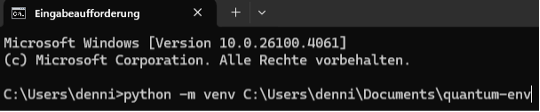
\includegraphics[width=1\linewidth]{Virtuelle Umgebung einrichten.png}
        \caption{Virtuelle Umgebung einrichten}
        \label{fig:enter-label}
    \end{figure}

 \item \textbf{Virtuelle Umgebung aktivieren}
    \begin{verbatim}
cd C:\Users\deinBenutzername\Documents\quantum-env
.\Scripts\activate
    \end{verbatim}
\textit{Diese Befehle wechseln in das Verzeichnis der virtuellen Umgebung und aktivieren sie.  Der Prompt zeigt danach den Namen der aktiven Umgebung an, was ein Zeichen dafür ist, dass alle weiteren Befehle lokal ausgeführt werden. }
    \begin{figure}
        \centering
        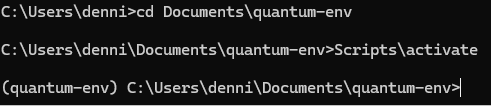
\includegraphics[width=1\linewidth]{Virtuelle Umgebung aktiviert.png}
        \caption{Virtuelle Umgebung aktiviert}
        \label{fig:enter-label}
    \end{figure}

    \item \textbf{pip-Version prüfen}
    \begin{verbatim}
pip --version
    \end{verbatim}
\textit{Dieser Befehl überprüft, ob der Python-Paketmanager \texttt{pip} korrekt installiert und aktiviert ist.  \texttt{pip} wird im nächsten Schritt zur Installation der Pakete verwendet. }
    \begin{figure}
        \centering
        \includegraphics[width=1\linewidth]{pip-version prüfen.png}
        \caption{pip-Version prüfen}
        \label{fig:enter-label}
    \end{figure}
\end{enumerate}

\subsubsection*{Installation der benötigten Pakete}

\begin{enumerate}
    \setcounter{enumi}{3} % Zähler für fortlaufende Liste
    \item \textbf{Qiskit installieren}
    \begin{verbatim}
pip install qiskit
    \end{verbatim}
\textit{Dieser Befehl installiert das Hauptpaket \texttt{qiskit}, das alle grundlegenden Funktionen zur Programmierung und Simulation von Quantencomputern enthält. }
    \begin{figure}
        \centering
        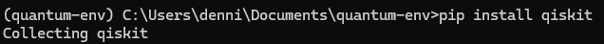
\includegraphics[width=1\linewidth]{Qiskit installieren.png}
        \caption{Qiskit installieren}
        \label{fig:enter-label}
    \end{figure}

    \item \textbf{Visualisierungsfunktionen hinzufügen (optional, empfohlen)}
    \begin{verbatim}
pip install qiskit[visualization]
    \end{verbatim}
\textit{Dieser Befehl installiert zusätzliche Bibliotheken zur grafischen Darstellung von Quanten-Schaltkreisen und Simulationsergebnissen, z.B. mit Matplotlib.  Dies ist notwendig bei Nutzung von Jupyter Notebook. }
    \begin{figure}
        \centering
        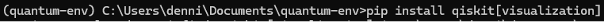
\includegraphics[width=1\linewidth]{Installation der Visualisierungsfunktion.png}
        \caption{Installation der Visualisierungsfunktion}
        \label{fig:enter-label}
    \end{figure}

    \item \textbf{IBM Runtime installieren (optional)}
    \begin{verbatim}
pip install qiskit-ibm-runtime
    \end{verbatim}
\textit{Dieser Befehl ermöglicht die Anbindung an echte Quantenhardware über IBMs Cloud-Umgebung.  Dies ist optional, aber hilfreich für fortgeschrittene Experimente. }
    \begin{figure}
        \centering
        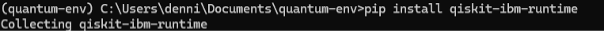
\includegraphics[width=1\linewidth]{Installation IBM Runtime.png}
        \caption{Installation IBM Runtime}
        \label{fig:enter-label}
    \end{figure}
\end{enumerate}

\subsubsection*{Jupyter Notebook nutzen}

\begin{enumerate}
    \setcounter{enumi}{6} % Zähler für fortlaufende Liste
    \item \textbf{Jupyter installieren}
    \begin{verbatim}
pip install jupyter
    \end{verbatim}
\textit{Dieser Befehl installiert Jupyter Notebook -- eine interaktive Umgebung, in der Python-Code, Visualisierungen und Textelemente kombiniert werden können. }
    \begin{figure}
        \centering
        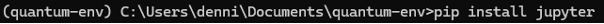
\includegraphics[width=1\linewidth]{Installation Jupyter Notebook.png}
        \caption{Installation Jupyter Notebook}
        \label{fig:enter-label}
    \end{figure}

    \item \textbf{Notebook starten}
    \begin{verbatim}
jupyter notebook
    \end{verbatim}
\textit{Dieser Befehl startet den Jupyter Notebook-Server und öffnet die Benutzeroberfläche im Webbrowser.  Hier können direkt interaktive Codebeispiele mit Qiskit ausgeführt werden. }
    \begin{figure}
        \centering
        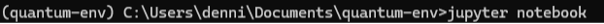
\includegraphics[width=1\linewidth]{Notebook starten.png}
        \caption{Notebook starten}
        \label{fig:enter-label}
    \end{figure}
\end{enumerate}

\subsubsection{Konstruktion des Grover Circuits:}


Um den Grover Algorithmus praktisch auf eine Quantencomputer umzusetzen, wird eine konkrete Konstruktion der Schaltung benötigt. Der Algorithmus setzt sich dabei aus 4 wesentlichen Komponenten zusammen: 
\begin{enumerate}
    \item  Initialisierung: Hierbei werden die Qubits in eine gleichmäßige Superposition gebracht
    \item Oracle: Im Oracle wird der gesuchte Zustand, welcher der Grover Algorithmus identifizieren soll, ausgewählt
    \item Diffusionsoperator: Der Diffusionsoperator verstärkt den Zustand des Oracle
    \item   Messung: Abgeschlossen wird der Algorithmus mit der Messung, um das Ergebnis zu erhalten. 
\end{enumerate}

Diese 4 Schritte können beliebig für eine beliebige Anzahl an Qubits angewendet werden. Im Folgenden werden die 4 Komponenten nochmals ausführlicher beschrieben. Das Ganze erfolgt jeweils mathematisch, konzeptionell und zusätzlich noch praktisch. Für den praktischen Teil wurde ein Grover Algorithmus mit Qiskit in Jupyter Notebooks implementiert und Codeausschnitte zeigen Schritt für Schritt die praktische Umsetzung.

\subsection*{Initialisierung}
Der Startzustand aller Qubits ist $\ket{0}$. Um eine gleichverteilte Superposition über alle Basiszustände der Qubits zu erzeugen, muss für jedes der Qubits ein Hadamard-Gate ($H$) angewendet werden. Für die Anzahl $n$ Qubits ergibt sich daraus folgender Zusammenhang:
$$
|\psi_0\rangle = H^{\otimes n}|0\rangle^{\otimes n} = \frac{1}{\sqrt{2^n}} \sum_{x=0}^{2^n-1} |x\rangle
$$
Der beschriebene Zustand bildet die Grundlage für die Amplitudenverstärkung von Grovers Algorithmus. Jede Lösung hat damit zunächst dieselbe Wahrscheinlichkeit. (Nielsen \& Chuang 2010, S.257)

Mit Qiskit in Jupyter Notebooks wird zunächst die `QuantumCircuit`-Bibliothek benötigt. Anschließend kann die Initialisierung, also der Ausgangspunkt für jeden Grover-Algorithmus, wie folgt in Qiskit umgesetzt werden:
\subsection*{Beispiel für 2 Qubits:}
\begin{verbatim}
from qiskit import QuantumCircuit

# Quantenschaltung mit 2 Qubits und 2 klassischen Bits erstellen
qc = QuantumCircuit(2, 2)

# Hadamard-Gate auf jedes Qubit anwenden
qc.h([0, 1])


\end{verbatim}


Das gewählte Beispiel ist für 2 Qubits, kann jedoch, wie bereits erwähnt, für die Anzahl $n$ Qubits beliebig erweitert werden.

\subsection*{Oracle}
Der nächste Schritt in der Implementierung des Grover-Algorithmus nennt sich Oracle. Bei Oracle handelt es sich um eine unitäre Operation $U_f$, welche den gesuchten Zustand $\ket{T}$ durch eine Phaseninversion der Qubits kenntlich macht. Das bedeutet, dass in diesem Schritt immer der gesuchte Zielzustand markiert wird. Dies erlaubt im Beispiel von 2 Qubits vier verschiedene Zielzustände: "00", "01", "10" und "11".

Dieser Zusammenhang wird wie folgt beschrieben:
$$
U_f \ket{x} = (-1)^{f(x)} \ket{x}
$$
Ein ideales Oracle wird formal wie folgt beschrieben:
$$
U_f \ket{x} = \begin{cases} -\ket{x} & \text{wenn } x \text{ der gesuchte Zustand ist} \\ \ket{x} & \text{sonst} \end{cases}
$$
Für die Standardversion des Grover-Algorithmus wird der Parameter $f(x)$ in der genannten Formel gesetzt, was zu folgender Formel führt:
$$
U_f \ket{x} = (-1)^{\delta_{x,T}} \ket{x}
$$
Die daraus entstehende Inversion lässt sich als eine Reflexion des Zustandsvektors im sogenannten Hilbertraum interpretieren. (Roy et al 2022, Grover 1996)

Zum besseren Verständnis, wie das Genannte mit Qiskit in Jupyter Notebooks umgesetzt wird, hier die Fortsetzung des Beispiels für 2 Qubits. Als Beispiel wird im Folgenden nun der Zielzustand $\ket{01}$ markiert.

Standardmäßig wirkt das CZ-Gate (Controlled-Z Gate) in Qiskit auf den Zustand $\ket{11}$. Wenn man nun einen der anderen genannten Zustände markieren möchte, muss man mit NOT-Gates (X-Gates) arbeiten, welche die Qubits so transformieren, dass der gewünschte Zielzustand vor dem CZ-Gate zum Zustand $\ket{11}$ wird und nach dem CZ-Gate wieder zurücktransformiert wird.

\subsection*{Zielzustand $\ket{01}$ markieren (Beispiel):}
Um den Zustand $\ket{01}$ zu markieren, invertieren wir das erste Qubit (Index 0) mit einem X-Gate, sodass aus $\ket{0}$ ein $\ket{1}$ wird. Das zweite Qubit (Index 1) bleibt $\ket{1}$. Somit wird aus $\ket{01}$ ein $\ket{11}$. Anschließend wenden wir das CZ-Gate an und invertieren das erste Qubit wieder zurück, um den Zustand wiederherzustellen.

\begin{verbatim}
# Oracle für den Zielzustand |01> erstellen
# Qubit 0 (links) ist 0, Qubit 1 (rechts) ist 1
# Um aus |01> ein |11> zu machen, muss Qubit 0 invertiert werden (X-Gate)

# X-Gate auf Qubit 0 anwenden (0 -> 1)
qc.x(0)
# CZ-Gate anwenden (wirkt auf |11>)
qc.cz(0, 1)
# X-Gate auf Qubit 0 zurückanwenden (1 -> 0)
qc.x(0)

# Schaltung zeichnen (optional)
# qc.draw('mpl')
\end{verbatim}
Mit dieser Vorgehensweise können beliebige Zielzustände auf einfache Weise realisiert werden, und das Ganze ohne zusätzliche Hilfs-Qubits. Das funktioniert auch für die Anzahl $n$ Qubits. (Roy et al, 2022)

---

\subsection*{Diffusionsoperator}
Der Diffusionsoperator, welcher auch häufig „Inversion about the mean“ genannt wird, verstärkt den im Oracle markierten Zielzustand, indem er alle Amplituden am Mittelwert reflektiert. Die Definition des Diffusionsoperators ist folgende:
$$
D = 2|\psi\rangle\langle\psi| - I
$$
Dabei steht der Parameter $|\psi\rangle$ für den gleichverteilten Zustand. Das entspricht aus geometrischer Sicht einer Spiegelung im Hilbertraum. Genau diese Operation ist für die Verstärkung des im Oracle markierten Zielzustands verantwortlich. Nach jeder Grover-Iteration bewirkt sie eine Rotation des Zustandsvektors um einen festen Winkel im Unterraum von markierten und unmarkierten Zuständen. (vgl. Grover 1996, Montanaro 2016).

In unserem gewählten Beispiel mit 2 Qubits kann der Diffusionsoperator in Qiskit wie folgt umgesetzt werden:
\begin{verbatim}
grover_circuit.h([0,1])   # Rücktransformation in H-Basis
grover_circuit.z([0,1])   # Phaseninversion aller Zustände
grover_circuit.cz([0,1])  # Inversion von |00> in H-Basis
grover_circuit.h([0,1])   # Zurück in ursrüngliche Basis
\end{verbatim}

Optional kann das auch mit dem `GroverOperator` aus der Qiskit-Bibliothek gelöst werden. Dieser kapselt Oracle und Diffusion und wird wie folgt umgesetzt:
\begin{verbatim}
from qiskit.circuit.library import GroverOperator
grover_op = GroverOperator (oracle=oracle)
\end{verbatim}

\subsection*{Messung}
Der abschließende Schritt im Grover Algorithmus ist die Messung. Diese folgt nach mehreren Iterationen von Oracle und Diffusion (typischerweise $\approx \frac{\pi}{4} \sqrt{2^n}$)
\begin{verbatim}
grover_circuit.measure_all()
\end{verbatim}
Diese überführt den quantenmechanischen Zustand in einen klassischen Bitstring. 
Die Wahrscheinlichkeit, bei der Messung den markierten Zustand zu erhalten ist nun maximal. Bei Benutzung der Simulation erfolgt diese Messung häufig mehrfach in sogenannten „shots“, um eine Wahrscheinlichkeitsverteilung zu erhalten. So lässt sich die Dominanz des gesuchten Zustands gegenüber der anderen Zustände statistisch nachweisen.

Die Konstruktion des Grover-Circuits ist modular und besteht wie beschrieben aus den genannten vier klar definierten Schritten. Mithilfe von Qiskit lassen sich diese Schritte präzise implementieren, debuggen und simulieren. Das kann sowohl für die theoretische Analyse als auch für praktische Experimente auf realen Quantencomputern verwendet werden.

\subsubsection{Ausführung auf Simulator (Qiskit Aer)}
\subsubsection{Visualisierung von Schaltkreis und Ergebnissen Konrad}

\setlength{\parindent}{0pt} % Keine Einrückung am Absatzanfang
\setlength{\parskip}{1em}   % Fügt einen vertikalen Abstand von 1em zwischen Absätzen ein

Ein zentrales Anliegen beim Verständnis und bei der Vermittlung von Quantenalgorithmen ist die Möglichkeit, deren Funktionsweise nicht nur abstrakt-mathematisch, sondern auch visuell nachvollziehen zu können. Das folgende Kapitel widmet sich der Visualisierung des Grover-Algorithmus anhand zweier Implementierungen – einmal mit zwei, einmal mit drei Qubits – unter Verwendung des Qiskit-Frameworks. Sowohl der Aufbau des Quanten-Schaltkreises als auch die Messergebnisse werden grafisch dargestellt und interpretiert.

\paragraph*{Visualisierung des Quantenschaltkreises}
\mbox{}

Für beide Varianten des Grover-Algorithmus wird der jeweilige Quanten-Schaltkreis mit der Methode QuantumCircuit.draw() visualisiert. Diese Darstellung erlaubt einen direkten Einblick in den logischen Aufbau des Algorithmus, insbesondere in die Abfolge und Wirkung der verschiedenen quantenmechanischen Operationen. Die Schaltkreise bestehen jeweils aus mehreren charakteristischen Abschnitten:
\begin{itemize}
    \item \textbf{Initialisierung:} Alle Qubits werden im Zustand $\ket{0}$    vorbereitet.
    \item \textbf{Superposition:} Durch Anwendung von Hadamard-Gattern wird eine gleichmäßige Überlagerung aller möglichen Basiszustände erzeugt.
    \item \textbf{Oracle:} Eine gezielte Phaseninversion kennzeichnet den gesuchten Zustand. Dieser Schritt implementiert die sogenannte „Markierung“ des Zielzustands.
    \item \textbf{Diffusion (Grover-Operator):} In einem weiteren Schritt wird der markierte Zustand durch Interferenz verstärkt. Dies geschieht durch Spiegelung an der Mittelwertachse aller Amplituden.
    \item \textbf{Messung:} Zum Abschluss des Algorithmus erfolgt eine Messung aller Qubits.
\end{itemize}
\noindent
Die nachstehenden Codeausschnitte zeigen, wie die Schaltkreise für beide
Varianten im Notebook erzeugt und angezeigt werden:

\begin{verbatim}
circuit.draw()
\end{verbatim}

  \begin{figure}
      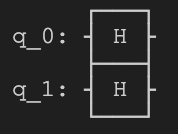
\includegraphics[width=0.25\linewidth]{circuit_superposition.png}
      \caption{Visualisierung des Schaltkreises (Superposition)}
      \label{fig:enter-label}
\end{figure}

\paragraph*{Visualisierung der Messergebnisse}
\mbox{}

Nach Ausführung des Algorithmus auf einem Quantensimulator – konkret dem QASM-Simulator von Qiskit – erfolgt die Analyse der Ergebnisse durch grafische Darstellung der Messausgänge.  Dabei wird die Methode \texttt{plot\_histogram()} verwendet, die ein Histogramm der gemessenen Zustände erzeugt.  Die Höhe der jeweiligen Balken repräsentiert die Häufigkeit (bzw. Wahrscheinlichkeit) eines bestimmten Bitmusters, das bei der Messung beobachtet wurde. 

Im Idealfall – das heißt, bei korrekter Funktionsweise des Orakels und des Grover-Operators – zeigt das Histogramm einen klar dominanten Peak beim Zielzustand.  Die Wahrscheinlichkeiten für alle anderen Zustände bleiben deutlich geringer.  Der gesuchte Zustand hebt sich somit durch quantenmechanische Verstärkung deutlich ab.  Der entsprechende Code zur Ergebnisvisualisierung lautet: 
\begin{verbatim}
plot_histogram(counts)
plt.show()
plot_histogram(counts)
plt.show()
\end{verbatim}

\begin{figure}
    \centering
    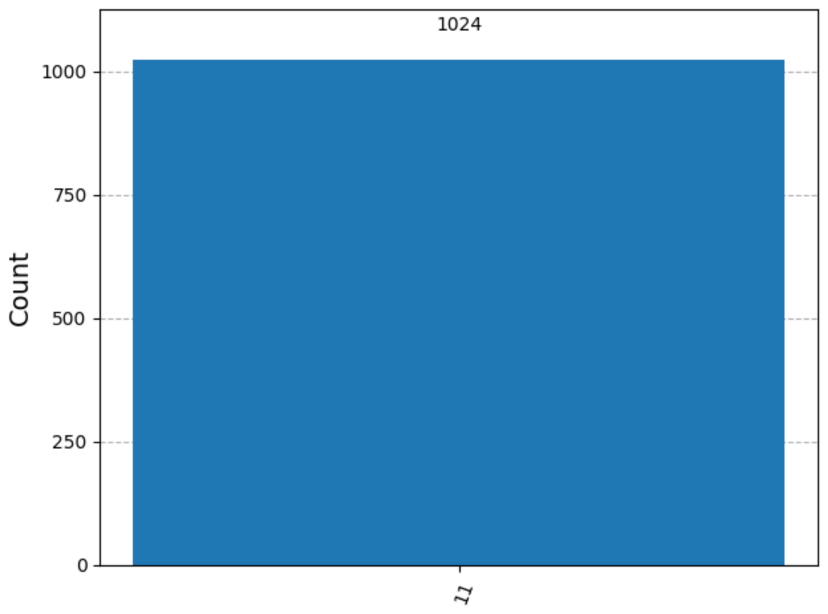
\includegraphics[width=1\linewidth]{Visualisierung der Messergebnisse.png}
    \caption{Visualisierung der Messergebnisse}
    \label{fig:enter-label}
\end{figure}

Die Kombination aus Schaltkreisvisualisierung und Ergebnisdarstellung bietet einen idealen Zugang zum Verständnis von Grovers Algorithmus.  Sie macht die Wirkung der einzelnen quantenlogischen Schritte nachvollziehbar und veranschaulicht das Prinzip der amplitudenbasierten Suche auf anschauliche Weise.  Solche Visualisierungen sind nicht nur didaktisch wertvoll, sondern auch essenziell für die Entwicklung und Analyse komplexerer Quantenalgorithmen in der Praxis. 

\clearpage % Fügt einen Seitenumbruch ein, um den nächsten Abschnitt auf einer neuen Seite zu beginnen

\subsubsection{Tests und Debugging-Hilfsmittel (z.\,B. Histogramme, Counts)}


\paragraph*{Tests und Debugging-Hilfsmittel}
\mbox{}

Bei der Entwicklung von Quantenalgorithmen spielt die systematische Überprüfung des Codes eine entscheidende Rolle, insbesondere im experimentellen Rahmen mit Frameworks wie Qiskit. Quantenprogramme sind nicht nur aufgrund ihrer Komplexität fehleranfällig, sondern verhalten sich auch häufig nicht intuitiv, da viele Zustände nicht direkt beobachtbar sind. Deshalb ist es essenziell, gezielt mit Tests, Zwischenergebnissen und Visualisierungen zu arbeiten, um Fehler zu erkennen und zu beheben.

\paragraph*{Schrittweise Entwicklung und Visualisierung}
\mbox{}

Im vorliegenden Notebook wurde der Grover-Algorithmus schrittweise aufgebaut, was eine erste Form des \enquote{Testens durch Design} darstellt. So wurden zunächst einzelne Operatoren und Zustände erzeugt, bevor sie in die Gesamtschaltung integriert wurden. Ein typisches Beispiel findet sich im Abschnitt zur 2-Qubit-Version:
\begin{verbatim}
def diffusion(circuit):
    circuit.h([0, 1])
    circuit.x([0, 1])
    circuit.h(1)
    circuit.cx(0, 1)
    circuit.h(1)
    circuit.x([0, 1])
    circuit.h([0, 1])
# Grover Circuit
grover_circ = QuantumCircuit(2)
grover_circ.h([0, 1])         # Superposition
oracle(grover_circ)           # Oracle anwenden
diffusion(grover_circ)        # Verstärkung
grover_circ.measure_all()
def diffusion(circuit):
    circuit.h([0, 1])
    circuit.x([0, 1])
    circuit.h(1)
    circuit.cx(0, 1)
    circuit.h(1)
    circuit.x([0, 1])
    circuit.h([0, 1])
# Grover Circuit
grover_circ = QuantumCircuit(2)
grover_circ.h([0, 1])         # Superposition
oracle(grover_circ)           # Oracle anwenden
diffusion(grover_circ)        # Verstärkung
grover_circ.measure_all()
\end{verbatim}
Durch das schrittweise Ergänzen der Gates kann bereits in frühen Phasen kontrolliert werden, ob jede Transformation wie gewünscht wirkt. Dies entspricht einem iterativen Debugging-Verfahren.

\paragraph*{Visualisierung als Debugging-Werkzeug}
\mbox{}

Wie im vorherigen Kapitel gezeigt, wird mit \texttt{draw()} der Schaltkreis visualisiert. Dies erfüllt nicht nur dokumentarische, sondern auch diagnostische Zwecke. Es kann dadurch überprüft werden, ob etwa das Oracle korrekt umgesetzt oder die Anzahl der Grover-Iterationen richtig gewählt wurde.
\subparagraph*{Beispiel:}
\begin{verbatim}
circuit.draw()
circuit.draw()
\end{verbatim}
Fehlende oder falsch platzierte Gates werden so unmittelbar sichtbar. Besonders hilfreich ist dies bei komplexeren Operatorfolgen wie in der 3-Qubit-Version.

\paragraph*{Ergebnisanalyse durch Histogramme}
\mbox{}

Ein sehr effektives Mittel zur Fehlererkennung ist die statistische Analyse der Ausgaben. Die mit \texttt{plot\_histogram()} erzeugten Verteilungen lassen Rückschlüsse auf das Verhalten des Algorithmus zu:
\begin{verbatim}
plot_histogram(result.get_counts())
plot_histogram(result.get_counts())
\end{verbatim}
Tritt der erwartete Peak beim Zielzustand nicht auf, kann dies auf einen Fehler im Oracle, in der Grover-Iteration oder in der Initialisierung hinweisen. Wurde beispielsweise ein falsches CZ-Gatter verwendet oder versehentlich eine falsche Qubit-Reihenfolge angesprochen, so verteilt sich die Wahrscheinlichkeitsmasse ungleichmäßig oder falsch.

\paragraph*{Fazit}
\mbox{}

Die Arbeit mit Quantenalgorithmen erfordert sowohl eine sorgfältige Teststrategie, klassische Softwareentwicklung aber auch eine strukturiertere Herangehensweise. Im Notebook werden bereits einfache Mittel wie Visualisierung, gezielte Zwischenschritte und Histogrammanalyse genutzt und sind eine große Hilfe beim Debugging. Für komplexere Algorithmen empfiehlt sich darüber hinaus der gezielte Einsatz von Statevector-Simulationen, Barrieren zur Strukturierung und die Ausgabe von Zwischenzuständen.

\subsection{Fazit und Ausblick}
\begin{itemize}
    \item Zusammenfassung der Entwicklungsschritte
    \item Stärken und Schwächen aktueller Toolchains
    \item Ausblick: Hybrid-Ansätze, komplexere Anwendungsfälle, Integration in klassische Softwarelandschaften
\end{itemize}

\printbibliography
